\documentclass[10pt,a4paper,oneside]{article}
\usepackage[utf8]{inputenc}
\usepackage[T1]{fontenc}
\usepackage{lmodern}
\usepackage{geometry}
\geometry{top=16mm, bottom=18mm, left=16mm, right=16mm}
\usepackage{amsmath,amssymb,amsfonts}
\usepackage{xcolor}
\usepackage{tcolorbox}
\usepackage{tikz}
\usetikzlibrary{shapes,arrows.meta,positioning,calc}
\usepackage{booktabs}
\usepackage{fancyhdr}
\usepackage{hyperref}
\usepackage{enumitem}
\usepackage{titlesec}

% Color Palette Definitions
\definecolor{primarynavy}{RGB}{26, 54, 93}       % Deep Navy
\definecolor{secondaryteal}{RGB}{13, 148, 136}   % Teal Accent
\definecolor{darkslate}{RGB}{45, 55, 72}        % Charcoal Text
\definecolor{lightbg}{RGB}{248, 250, 252}        % Soft Background
\definecolor{accentblue}{RGB}{49, 130, 206}      % Bright Blue
\definecolor{warmgold}{RGB}{180, 83, 9}          % Dark Amber/Gold
\definecolor{crimsonred}{RGB}{197, 48, 48}       % Hazard Red
\definecolor{forestgreen}{RGB}{47, 133, 90}      % Protocol Green
\definecolor{royalpurple}{RGB}{107, 70, 193}     % Mechanism Purple

% Custom TColorBox Styles (Compact & Concise)
\newtcolorbox{conceptbox}[1]{
    colback=lightbg,
    colframe=primarynavy,
    fonttitle=\bfseries\color{white},
    coltitle=white,
    colbacktitle=primarynavy,
    title=#1,
    arc=1.2mm,
    boxrule=0.8pt,
    top=2mm, bottom=2mm, left=3mm, right=3mm
}

\newtcolorbox{mechanismbox}[1]{
    colback=lightbg,
    colframe=royalpurple,
    fonttitle=\bfseries\color{white},
    coltitle=white,
    colbacktitle=royalpurple,
    title=#1,
    arc=1.2mm,
    boxrule=0.8pt,
    top=2mm, bottom=2mm, left=3mm, right=3mm
}

\newtcolorbox{hazardbox}[1]{
    colback=lightbg,
    colframe=crimsonred,
    fonttitle=\bfseries\color{white},
    coltitle=white,
    colbacktitle=crimsonred,
    title=#1,
    arc=1.2mm,
    boxrule=0.8pt,
    top=2mm, bottom=2mm, left=3mm, right=3mm
}

\newtcolorbox{protocolbox}[1]{
    colback=lightbg,
    colframe=forestgreen,
    fonttitle=\bfseries\color{white},
    coltitle=white,
    colbacktitle=forestgreen,
    title=#1,
    arc=1.2mm,
    boxrule=0.8pt,
    top=2mm, bottom=2mm, left=3mm, right=3mm
}

\newtcolorbox{mnemonicbox}[1]{
    colback=lightbg,
    colframe=warmgold,
    fonttitle=\bfseries\color{white},
    coltitle=white,
    colbacktitle=warmgold,
    title=#1,
    arc=1.2mm,
    boxrule=0.8pt,
    top=2mm, bottom=2mm, left=3mm, right=3mm
}

% Header and Footer Formatting
\pagestyle{fancy}
\fancyhf{}
\fancyhead[L]{\small\color{primarynavy}\textbf{CHEMV51: Food Chemistry \& Adulteration}}
\fancyhead[R]{\small\color{secondaryteal}Concise Notes: Common Adulterants \quad \bfseries\color{primarynavy}\thepage}
\fancyfoot{}
\renewcommand{\headrulewidth}{0.5pt}

% Section Titles Styling
\titleformat{\section}
  {\color{primarynavy}\normalfont\large\bfseries}{\thesection}{0.8em}{}[\titlerule]
\titleformat{\subsection}
  {\color{secondaryteal}\normalfont\normalsize\bfseries}{\thesubsection}{0.8em}{}

\setlist{itemsep=0.15em, topsep=0.2em, parsep=0.1em}

\hypersetup{
    colorlinks=true,
    linkcolor=primarynavy,
    urlcolor=accentblue,
    citecolor=forestgreen,
    pdftitle={Concise Notes: Common Adulterants in Food},
    pdfauthor={Chemistry Department}
}

\begin{document}

% -----------------------------------------------------------------------------
% COMPACT HEADER TITLE BLOCK
% -----------------------------------------------------------------------------
\begin{center}
    {\large \bfseries \color{secondaryteal} COURSE CHEMV51: FOOD CHEMISTRY \& ADULTERATION}\\[0.15cm]
    {\LARGE \bfseries \color{primarynavy} Module 2: Common Adulterants in Food}\\[0.15cm]
    {\normalsize \color{darkslate}\textbf{Concise Exam Notes: Mechanisms, Reactions, Tests, Mnemonics \& Solved Questions}}\\[0.25cm]
    \rule{\linewidth}{1.2pt}
\end{center}

\vspace{-0.2cm}

% =============================================================================
% SECTION 1: OVERVIEW & MACRO FLOWCHART
% =============================================================================
\section{Overview of Food Adulteration}

\textbf{Definition:} Fraudulent addition of substandard/toxic substances or removal of vital nutritional constituents from food commodities to maximize illicit profit or conceal spoilage.
\begin{itemize}
    \item \textbf{Intentional (EMA):} Deliberate commercial fraud (watering milk, urea, Vanaspati in ghee, synthetic colorants).
    \item \textbf{Incidental:} Unintentional contamination (ergot mold sclerotia, pesticide residues, heavy metal leaching).
\end{itemize}

\vspace{0.2cm}

\begin{center}
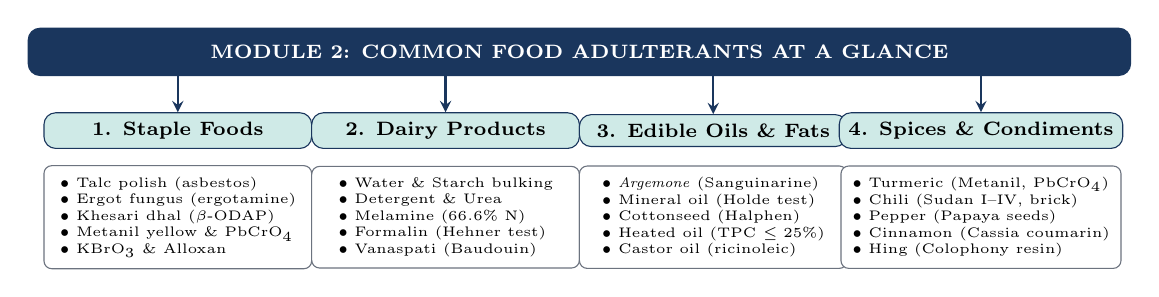
\begin{tikzpicture}[
    box/.style={rectangle, draw=primarynavy, fill=lightbg, rounded corners=1.5mm, text centered, font=\scriptsize\bfseries},
    detailbox/.style={rectangle, draw=darkslate!70, fill=white, rounded corners=1mm, font=\tiny, align=left, inner sep=4pt},
    arrow/.style={thick, ->, >=stealth, color=primarynavy}
]
    \node[box, fill=primarynavy, text=white, minimum width=14cm, minimum height=0.6cm] (root) at (0, 0) {MODULE 2: COMMON FOOD ADULTERANTS AT A GLANCE};
    
    \node[box, fill=secondaryteal!20, minimum width=3.4cm] (b1) at (-5.1, -1.0) {1. Staple Foods};
    \node[box, fill=secondaryteal!20, minimum width=3.4cm] (b2) at (-1.7, -1.0) {2. Dairy Products};
    \node[box, fill=secondaryteal!20, minimum width=3.4cm] (b3) at (1.7, -1.0) {3. Edible Oils \& Fats};
    \node[box, fill=secondaryteal!20, minimum width=3.4cm] (b4) at (5.1, -1.0) {4. Spices \& Condiments};
    
    \draw[arrow] (-5.1, -0.3) -- (b1.north);
    \draw[arrow] (-1.7, -0.3) -- (b2.north);
    \draw[arrow] (1.7, -0.3) -- (b3.north);
    \draw[arrow] (5.1, -0.3) -- (b4.north);
    
    \node[detailbox, minimum width=3.4cm] at (-5.1, -2.1) {$\bullet$ Talc polish (asbestos)\\$\bullet$ Ergot fungus (ergotamine)\\$\bullet$ Khesari dhal ($\beta$-ODAP)\\$\bullet$ Metanil yellow \& $\mathrm{PbCrO_4}$\\$\bullet$ $\mathrm{KBrO_3}$ \& Alloxan};
    \node[detailbox, minimum width=3.4cm] at (-1.7, -2.1) {$\bullet$ Water \& Starch bulking\\$\bullet$ Detergent \& Urea\\$\bullet$ Melamine ($66.6\%\ \mathrm{N}$)\\$\bullet$ Formalin (Hehner test)\\$\bullet$ Vanaspati (Baudouin)};
    \node[detailbox, minimum width=3.4cm] at (1.7, -2.1) {$\bullet$ \textit{Argemone} (Sanguinarine)\\$\bullet$ Mineral oil (Holde test)\\$\bullet$ Cottonseed (Halphen)\\$\bullet$ Heated oil (TPC $\le 25\%$)\\$\bullet$ Castor oil (ricinoleic)};
    \node[detailbox, minimum width=3.4cm] at (5.1, -2.1) {$\bullet$ Turmeric (Metanil, $\mathrm{PbCrO_4}$)\\$\bullet$ Chili (Sudan I--IV, brick)\\$\bullet$ Pepper (Papaya seeds)\\$\bullet$ Cinnamon (Cassia coumarin)\\$\bullet$ Hing (Colophony resin)};
\end{tikzpicture}
\end{center}

\vspace{-0.2cm}

% =============================================================================
% SECTION 2: ADULTERATION IN STAPLE FOODS
% =============================================================================
\section{Adulteration in Staple Foods (Grains, Pulses, Flours)}

\subsection{Grains (Wheat, Rice, Bajra)}
\begin{itemize}[leftmargin=*]
    \item \textbf{Talc / Soapstone ($\mathrm{Mg_3Si_4O_{10}(OH)_2}$):} Imparts white shine to rice/pulses. Stomach irritant; often carries tremolite asbestos fibers (IARC Group 1). \textit{Detection:} High acid-insoluble ash ($>0.5\%$).
    \item \textbf{Mineral Oil Glaze:} Non-saponifiable hydrocarbons prevent moisture loss; blocks absorption of fat-soluble vitamins (A, D, E, K). \textit{Detection:} Bright blue-violet fluorescence under UV ($365\text{ nm}$).
    \item \textbf{Ergot Sclerotia (\textit{Claviceps purpurea}):} Purplish-black fungal bodies contaminating rye, wheat, bajra. Contain peptide alkaloids (\textbf{Ergotamine}, \textbf{Ergocristine}) that cause intense peripheral vasoconstriction $\rightarrow$ \textbf{Ergotism / St. Anthony's Fire} (dry gangrene of digits, severe burning, uterine contractions/abortions).
    \begin{protocolbox}{Salt Floatation Test for Ergot}
    Suspend grains in a \textbf{$20\%\ \mathrm{NaCl}$ brine solution} (sp. gr. $\approx 1.15$). Clean sound grains sink; light spongy ergot sclerotia float on the surface and are skimmed off.
    \end{protocolbox}
    \item \textbf{Datura Seeds:} Kidney-shaped black seeds with tropane alkaloids (\textbf{Hyoscyamine, Scopolamine}). Anticholinergic toxidrome (mydriasis, extreme tachycardia, dry mouth, delirium).
\end{itemize}

\subsection{Pulses (Legumes)}
\begin{mechanismbox}{Khesari Dhal (*Lathyrus sativus*) and Neurolathyrism}
\textbf{Fraud:} Blended into expensive Arhar/Toor dhal (*Cajanus cajan*) and Chana dhal.\\
\textbf{Morphology:} Wedge-shaped, trapezoidal, slant-cut seeds vs. round Arhar dhal.\\
\textbf{Neurotoxin:} $\beta\text{-}N\text{-oxalyl-}\alpha,\beta\text{-diaminopropionic acid}$ (\textbf{$\beta$-ODAP / BOAA}).
$$\mathrm{HOOC-C(=O)-NH-CH_2-CH(NH_2)-COOH}$$
\textbf{Mechanism:} Structural analogue of glutamate; hyper-activates post-synaptic **AMPA receptors** on Betz cells and spinal motor neurons $\rightarrow$ massive $\mathrm{Ca}^{2+}$ influx $\rightarrow$ oxidative motor neuron lysis $\rightarrow$ \textbf{Neurolathyrism} (irreversible spastic paraplegia of legs, scissoring gait).\\
\textbf{Detoxification:} $\beta$-ODAP is water-soluble; boiling seeds in water ($1:10$) for 60 min and draining removes $>85\%$ toxin.
\end{mechanismbox}

\begin{itemize}[leftmargin=*]
    \item \textbf{Metanil Yellow:} Synthetic monoazo dye added to color inferior pulses and turmeric. Cleaved by gut azoreductases into toxic \textbf{$p$-aminodiphenylamine} (causes testicular seminiferous tubule atrophy).
    $$\text{Extract with water} + \text{conc. } \mathrm{HCl} \longrightarrow \textbf{Persistent Magenta / Pink-Red Color} \quad (\lambda_{\text{max}} \approx 530\text{ nm, quinoid dication})$$
    \item \textbf{Lead Chromate ($\mathrm{PbCrO_4}$):} Industrial paint pigment on turmeric and pulses. $\mathrm{Pb}^{2+}$ inhibits $\delta$-ALAD in heme synthesis $\rightarrow$ microcytic anemia, saturnism, and encephalopathy. \textit{Detection:} Ash sample $+\ \mathrm{HNO_3} +\ \mathrm{KI} \rightarrow$ \textbf{golden-yellow $\mathrm{PbI_2}\downarrow$}.
\end{itemize}

\subsection{Flours (Atta, Maida)}
\begin{itemize}[leftmargin=*]
    \item \textbf{Potassium Bromate ($\mathrm{KBrO_3}$):} Strong oxidizing agent. Converts gluten thiol ($-\mathrm{SH}$) to disulfide bridges ($-\mathrm{S-S-}$):
    $$2\ \text{Gluten-SH} + \mathrm{KBrO_3 \longrightarrow \text{Gluten-S-S-Gluten} + KBr + H_2O}$$
    Inflates bread loaf volume. IARC 2B carcinogen (renal cell tumors); banned by FSSAI. Spotting flour with $0.5\%\ \mathrm{KI} + 2\mathrm{M}\ \mathrm{HCl}$ gives **black-purple spots** ($\mathrm{I_2}$ + starch).
    \item \textbf{Alloxan ($\mathrm{C_4H_2N_2O_4}$):} Bleaching byproduct in maida. Enters pancreatic $\beta$-cells via **GLUT2** $\rightarrow$ reduced to dialuric acid $\rightarrow$ generates cytotoxic hydroxyl radicals ($\mathrm{\cdot OH}$) via Fenton reaction $\rightarrow$ necrotic $\beta$-cell death $\rightarrow$ **Type-1 Diabetes**.
\end{itemize}

\newpage

% =============================================================================
% SECTION 3: ADULTERATION IN DAIRY PRODUCTS
% =============================================================================
\section{Adulteration in Dairy Products}

\subsection{Synthetic Milk Formulation \& Rapid Screening Tests}
Synthetic milk is prepared using vegetable oil (fat phase), detergent/LAS (emulsifier/foam), urea (specific gravity/NPN), neutralizers ($\mathrm{NaOH, NaHCO_3}$ to prevent boiling curdling), starch (SNF/viscosity), and formalin (preservative).

\begin{center}
\small
\begin{tabular}{@{}p{3.0cm} p{5.5cm} p{8.5cm}@{}}
\toprule
\textbf{Adulterant} & \textbf{Rapid Chemical Test \& Reagents} & \textbf{Diagnostic Positive Observation \& Note} \tabularnewline
\midrule
\textbf{Water Dilution} & Lactometer Reading / Cryoscopy & Lactometer $<28$ at $20^\circ\text{C}$; freezing point shifted toward $0^\circ\text{C}$ (norm: $-0.540^\circ\text{C}$). \tabularnewline
\textbf{Starch / Dextrin} & $1\%\ \mathrm{I_2 / KI}$ Iodine Reagent & **Intense deep blue-black color** (polyiodide-amylose complex). \tabularnewline
\textbf{Urea} & DMAB reagent ($p$-dimethylaminobenzaldehyde) & **Intense bright yellow-green color** (pure milk gives faint yellow). \tabularnewline
\textbf{Detergents} & Methylene Blue dye $+$ Chloroform shake & **Lower chloroform layer turns blue** (anionic surfactant complex). \tabularnewline
\textbf{Neutralizers} & $0.1\%$ Rosalic Acid in ethanol & **Rose-red color** (pure milk gives pale brownish-orange). \tabularnewline
\textbf{Formalin ($37\%$)} & **Hehner's Test** (conc. $\mathrm{H_2SO_4} + \text{trace }\mathrm{Fe}^{3+}$) & **Violet / purple ring at interface** (condensation with tryptophan in casein). \tabularnewline
\bottomrule
\end{tabular}
\end{center}

\vspace{0.1cm}

\begin{minipage}[c]{0.52\textwidth}
\begin{mechanismbox}{Melamine Triazine Fraud ($\mathrm{C_3H_6N_6}$)}
\textbf{Analytical Flaw:} Melamine has **$66.6\%$ nitrogen by mass**. Standard Kjeldahl testing calculates crude protein as $\% N \times 6.38$, reading melamine as protein ($1\text{ g}$ melamine in $1\text{ L}$ watered milk inflates protein by $+4.25\%$).\\
\textbf{Toxicity:} Melamine pairs via hydrogen bonding with cyanuric acid to form insoluble **[Melamine $\cdot$ Cyanuric Acid]** co-crystalline spherulites ($K_{\text{sp}} \approx 10^{-9}\ \mathrm{M^2}$) in renal tubules $\rightarrow$ **Obstructive urolithiasis and acute kidney injury**.
\end{mechanismbox}
\end{minipage}
\hfill
\begin{minipage}[c]{0.45\textwidth}
\centering
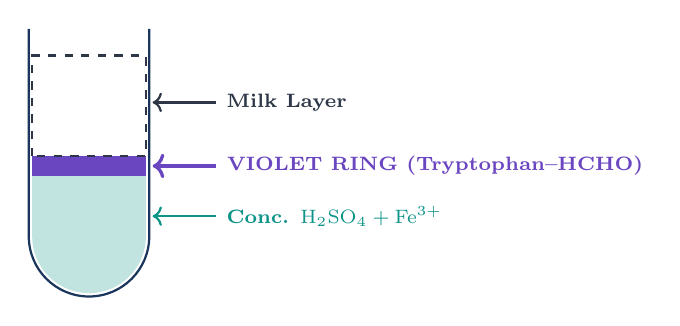
\begin{tikzpicture}[scale=0.85]
    \draw[thick, primarynavy] (0, 3.6) -- (0, 0.5) arc(180:360:0.9cm) -- (1.8, 3.6);
    \fill[secondaryteal!25] (0.05, 0.5) arc(180:360:0.85cm) -- (1.75, 1.4) -- (0.05, 1.4) -- cycle;
    \fill[royalpurple] (0.05, 1.4) rectangle (1.75, 1.7);
    \fill[white] (0.05, 1.7) rectangle (1.75, 3.2);
    \draw[thick, dashed, darkslate] (0.05, 1.7) rectangle (1.75, 3.2);
    
    \draw[<-, thick, darkslate] (1.85, 2.5) -- (2.8, 2.5) node[right, font=\scriptsize\bfseries] {Milk Layer};
    \draw[<-, very thick, royalpurple] (1.85, 1.55) -- (2.8, 1.55) node[right, font=\scriptsize\bfseries, text=royalpurple] {VIOLET RING (Tryptophan--HCHO)};
    \draw[<-, thick, secondaryteal] (1.85, 0.8) -- (2.8, 0.8) node[right, font=\scriptsize\bfseries] {Conc. $\mathrm{H_2SO_4} + \mathrm{Fe}^{3+}$};
\end{tikzpicture}
{\small\bfseries Figure: Hehner's Test Tube for Formalin}
\end{minipage}

\subsection{Ghee and Butter Adulteration}
\begin{itemize}[leftmargin=*]
    \item \textbf{Vanaspati (Hydrogenated Oil) in Ghee:} Catalytic partial hydrogenation ($\mathrm{H_2/Ni}$) converts cis-unsaturated fats to saturated and \textit{trans}-fatty acids (\textbf{elaidic acid}). Lowers Reichert-Meissl (RM) value from normal $26 - 32$ to $<1.0$.
    \item \textbf{Baudouin Test:} Vanaspati legally contains $5\%$ sesame oil. Conc. $\mathrm{HCl}$ hydrolyzes sesame **sesamolin** to **sesamol**, which condenses with added **furfural** $\rightarrow$ **crimson-rose red color** in acid layer. Pure ghee yields no color.
\end{itemize}

% =============================================================================
% SECTION 4: EDIBLE OILS AND FATS
% =============================================================================
\section{Adulteration in Edible Oils and Fats}

\begin{hazardbox}{*Argemone mexicana* Poisoning (Epidemic Dropsy)}
\textbf{Seeds:} Smooth round mustard seeds vs. rough, pitted *Argemone* seeds with a **pointed apical beak**.\\
\textbf{Toxic Alkaloid:} **Sanguinarine** and Dihydrosanguinarine.\\
\textbf{Pathophysiology:} (1) Sanguinarine inhibits membrane **$\mathrm{Na^+/K^+}$-ATPase** $\rightarrow$ cellular $\mathrm{Na^+}$ retention and edema; (2) Hyper-activates **eNOS**, releasing massive **Nitric Oxide ($\mathrm{NO}$)** $\rightarrow$ systemic capillary hyperpermeability and fluid extravasation.\\
\textbf{Clinical Signs (Dropsy):} Bilateral lower extremity pitting edema with erythema, secondary open-angle glaucoma (trabecular capillary dilation), and high-output congestive heart failure.\\
\textbf{Detection:} (a) Oil $+$ conc. $\mathrm{HNO_3} \rightarrow$ **crimson-red ring**; (b) Saponified oil $+\ \mathrm{HCl} +\ \mathrm{FeCl_3} \rightarrow$ reddish-brown needle crystals; (c) TLC under UV ($366\text{ nm}$) $\rightarrow$ bright **golden-yellow/orange fluorescence** ($R_f \approx 0.42$).
\end{hazardbox}

\begin{itemize}[leftmargin=*]
    \item \textbf{Mineral Oil (Holde's Saponification Test):} Vegetable oils saponify with alcoholic $\mathrm{KOH}$ to water-soluble soaps. Petroleum hydrocarbons cannot saponify; adding boiling water causes **persistent milky turbidity**.
    \item \textbf{Cottonseed Oil (Halphen Test):} Contains toxic **gossypol** and cyclopropenoid fatty acids (malvalic, sterculic). Heated with $1\%$ sulfur in $\mathrm{CS_2}$ at $110^\circ\text{C}$ produces a persistent **deep rose-red color**.
    \item \textbf{Used Cooking Oil (UCO):} Deep frying ($>180^\circ\text{C}$) forms toxic aldehydes (acrolein, 4-HNE) and polymers. \textbf{FSSAI statutory threshold: Total Polar Compounds (TPC) $\le 25\%$}. Oil exceeding $25\%$ TPC is banned.
\end{itemize}

% =============================================================================
% SECTION 5: SPICES AND CONDIMENTS
% =============================================================================
\section{Adulteration in Spices and Condiments}

\begin{center}
\small
\begin{tabular}{@{}p{3.0cm} p{4.0cm} p{4.5cm} p{5.5cm}@{}}
\toprule
\textbf{Spice Matrix} & \textbf{Common Adulterants} & \textbf{Diagnostic Screening Test} & \textbf{Toxicology / Hazard Impact} \tabularnewline
\midrule
\textbf{Turmeric Powder} & Metanil Yellow, Lead Chromate & Conc. $\mathrm{HCl} \rightarrow$ magenta-red; $\mathrm{KI} \rightarrow$ yellow $\mathrm{PbI_2}\downarrow$ & Testicular damage, saturnism, anemia. \tabularnewline
\textbf{Chili Powder} & Sudan I--IV dyes, brick dust, red lead & Brick settles in water; Sudan detected by TLC & Sudan dyes are genotoxic IARC carcinogens. \tabularnewline
\textbf{Black Pepper} & Dried Papaya Seeds & \textbf{Floatation:} Papaya seeds float; pepper sinks & Ingestion of toxic carpine alkaloid. \tabularnewline
\textbf{Cinnamon} & Cassia Bark (*C. cassia*) & Cassia turns deep blue with iodine decoction & Cassia has **Coumarin ($0.2-1\%$)** $\rightarrow$ liver necrosis. \tabularnewline
\textbf{Asafoetida (Hing)} & Colophony (pine) resin, gypsum & Pure forms milky emulsion; burns cleanly & Colophony causes contact dermatitis \& ulcers. \tabularnewline
\bottomrule
\end{tabular}
\end{center}

\begin{mechanismbox}{Ceylon Cinnamon vs. Cassia Bark}
True Ceylon cinnamon consists of delicate, multilayered, paper-thin parchment quills with safe coumarin ($<0.004\%$). Cassia consists of thick ($1-3\text{ mm}$), single woody hollow rolls containing **$0.2-1.0\%$ Coumarin**. Coumarin is epoxidized by CYP2A6 into **3,4-coumarin epoxide**, causing centrilobular liver necrosis and kidney injury.
\end{mechanismbox}

\newpage

% =============================================================================
% SECTION 6: MASTER MNEMONICS
% =============================================================================
\section{Master Mnemonics for Fast Exam Recall}

\begin{mnemonicbox}{High-Yield Exam Mnemonics}
\begin{itemize}[leftmargin=*]
    \item \textbf{D-R-O-P-S-Y (Argemone / Sanguinarine):}  
    \textbf{D}ilation of capillaries (via $\mathrm{NO}$) $\bullet$ \textbf{R}edness/rash $\bullet$ \textbf{O}xidative phosphorylation uncoupled $\bullet$ \textbf{P}itting lower limb edema $\bullet$ \textbf{S}anguinarine inhibits $\mathrm{Na^+/K^+}$-ATPase $\bullet$ \textbf{Y}ellow UV fluorescence on TLC.
    \item \textbf{F-U-N-D-S (Milk Rapid Screening Tests):}  
    \textbf{F}ormalin (Hehner's violet ring) $\bullet$ \textbf{U}rea (DMAB yellow-green) $\bullet$ \textbf{N}eutralizers (Rosalic acid rose-red) $\bullet$ \textbf{D}etergent (Methylene blue chloroform layer) $\bullet$ \textbf{S}tarch (Iodine deep blue).
    \item \textbf{B-A-U-D-O-U-I-N (Vanaspati in Ghee):}  
    \textbf{B}y-product sesamol $\bullet$ \textbf{A}cid ($\mathrm{HCl}$) hydrolysis $\bullet$ \textbf{U}nsaponifiable sesame oil $\bullet$ \textbf{D}ialdehyde: Furfural $\bullet$ \textbf{O}verlay turns \textbf{Rose-Red} $\bullet$ \textbf{I}ndicates Vanaspati $\bullet$ \textbf{N}egative in pure ghee.
    \item \textbf{O-D-A-P (Khesari Dhal Neurotoxin):}  
    \textbf{O}xalyl radical ($\beta$-ODAP / BOAA) $\bullet$ \textbf{D}epolarization via AMPA $\bullet$ \textbf{A}rhar dhal substituted $\bullet$ \textbf{P}araplegia (Neurolathyrism).
\end{itemize}
\end{mnemonicbox}

% =============================================================================
% SECTION 7: SOLVED QUESTION BANK & NUMERICALS
% =============================================================================
\section{High-Yield Solved Question Bank}

\subsection{Multiple Choice Questions (MCQs)}
\begin{enumerate}[leftmargin=*]
    \item Which neurotoxin in Khesari Dhal causes neurolathyrism?  
    (a) Sanguinarine \quad (b) $\beta$-ODAP / BOAA \quad (c) Coumarin \quad (d) Alloxan \hfill \textbf{[Ans: (b)]}
    \item In Hehner's test for formalin in milk, the violet ring forms by reaction with which amino acid?  
    (a) Methionine \quad (b) Cysteine \quad (c) Tryptophan \quad (d) Phenylalanine \hfill \textbf{[Ans: (c)]}
    \item Baudouin test detects Vanaspati in ghee via condensation of furfural with:  
    (a) Gossypol \quad (b) Sesamol \quad (c) Sanguinarine \quad (d) Ricinoleic acid \hfill \textbf{[Ans: (b)]}
    \item Primary enzyme inhibited by Sanguinarine in Epidemic Dropsy is:  
    (a) Acetylcholinesterase \quad (b) $\mathrm{Na^+/K^+}$-ATPase \quad (c) Cytochrome c oxidase \hfill \textbf{[Ans: (b)]}
    \item Melamine is added to milk to deceptively inflate:  
    (a) RM value \quad (b) Specific gravity \quad (c) Crude protein in Kjeldahl test \hfill \textbf{[Ans: (c)]}
    \item Metanil yellow in pulses is confirmed when concentrated $\mathrm{HCl}$ gives:  
    (a) Emerald green \quad (b) Persistent magenta-pink \quad (c) White turbidity \hfill \textbf{[Ans: (b)]}
    \item Holde's test detects mineral oil in vegetable oil based on:  
    (a) Persistent milky turbidity after saponification \quad (b) Acidity \quad (c) Fluorescence \hfill \textbf{[Ans: (a)]}
    \item Toxic component in Cassia bark that induces centrilobular liver necrosis is:  
    (a) Eugenol \quad (b) Coumarin \quad (c) Cinnamaldehyde \quad (d) Safrole \hfill \textbf{[Ans: (b)]}
    \item Statutory FSSAI maximum limit of Total Polar Compounds (TPC) in frying oil is:  
    (a) $10\%$ \quad (b) $15\%$ \quad (c) $25\%$ \quad (d) $40\%$ \hfill \textbf{[Ans: (c)]}
    \item Papaya seeds are separated from genuine black pepper because they:  
    (a) Sink in water \quad (b) Float on water/alcohol \quad (c) Turn blue with iodine \hfill \textbf{[Ans: (b)]}
\end{enumerate}

\subsection{Short Answer Questions (SAQs)}
\begin{itemize}[leftmargin=*]
    \item \textbf{Q1. Explain the Baudouin Test principle.}  
    \textit{Ans:} Vanaspati contains mandated $5\%$ sesame oil. Concentrated $\mathrm{HCl}$ hydrolyzes sesame sesamolin into sesamol. Sesamol condenses with added furfural in acid medium to yield an intense, persistent \textbf{crimson-rose red} quinoid dye. Pure ghee gives no color.
    \item \textbf{Q2. What causes Epidemic Dropsy?}  
    \textit{Ans:} Consumption of mustard oil adulterated with \textit{Argemone mexicana} oil containing \textbf{Sanguinarine}. Sanguinarine inhibits $\mathrm{Na^+/K^+}$-ATPase and triggers excess Nitric Oxide release, causing bilateral lower-limb pitting edema, secondary open-angle glaucoma, and cardiac failure.
    \item \textbf{Q3. Why does Kjeldahl test fail to detect Melamine?}  
    \textit{Ans:} Kjeldahl converts all nitrogen to $(\mathrm{NH_4})_2\mathrm{SO_4}$ and multiplies by $6.38$. Because melamine has $66.6\%$ nitrogen, it deceptively inflates apparent protein without distinguishing peptide bonds from triazine rings.
    \item \textbf{Q4. How to differentiate Ceylon Cinnamon from Cassia?}  
    \textit{Ans:} Ceylon cinnamon has delicate multilayered parchment quills with safe coumarin ($<0.004\%$). Cassia has thick, woody single hollow rolls containing high \textbf{hepatotoxic Coumarin ($0.2-1.0\%$)}.
    \item \textbf{Q5. Role of Potassium Bromate in flour.}  
    \textit{Ans:} $\mathrm{KBrO_3}$ oxidizes gluten cysteine $-\mathrm{SH}$ to disulfide crosslinks ($-\mathrm{S-S-}$), trapping $\mathrm{CO_2}$ and inflating bread volume. It is a banned IARC 2B renal carcinogen.
\end{itemize}

\subsection{Solved Quantitative Numericals}
\begin{conceptbox}{Numerical 1: Kjeldahl Melamine Protein Correction}
\textbf{Problem:} Milk powder has $0.7844\%$ total nitrogen. (a) Find apparent protein ($F = 6.38$). (b) If $0.15\%$ of powder weight is Melamine ($66.63\%\ \mathrm{N}$), calculate true protein.\\
\textbf{Solution:}
\begin{enumerate}
    \item $\text{Apparent Crude Protein} = 0.7844\% \times 6.38 = \mathbf{5.004\%}$.
    \item Nitrogen contributed by $0.15\text{ g}$ melamine per $100\text{ g} = 0.15 \times 0.6663 = 0.0999\%\ \mathrm{N}$.\\
    $\text{True Dairy Nitrogen} = 0.7844\% - 0.0999\% = 0.6845\%$.
    \item $\mathbf{\text{True Protein}} = 0.6845\% \times 6.38 = \mathbf{4.367\%}$. *(Melamine inflated protein by $+14.6\%$)*.
\end{enumerate}
\end{conceptbox}

\begin{conceptbox}{Numerical 2: Reichert-Meissl (RM) Value Dilution}
\textbf{Problem:} Suspected cow ghee has an RM value of $14.5$. Pure ghee RM is $28.0$ and Vanaspati RM is $0.6$. Calculate $\%$ Vanaspati.\\
\textbf{Solution:}
$$\% \text{Vanaspati} = \frac{RM_{\text{pure}} - RM_{\text{sample}}}{RM_{\text{pure}} - RM_{\text{vanaspati}}} \times 100 = \frac{28.0 - 14.5}{28.0 - 0.6} \times 100 = \frac{13.5}{27.4} \times 100 = \mathbf{49.27\%}$$
\end{conceptbox}

\newpage

% =============================================================================
% SECTION 8: MASTER QUICK REVISION SHEET & CHECKLIST
% =============================================================================
\section{Master Quick Revision Sheet \& Pre-Exam Checklist}

\begin{center}
\small
\begin{tabular}{@{}p{3.2cm} p{3.8cm} p{10.0cm}@{}}
\toprule
\textbf{Food Matrix} & \textbf{Target Adulterant} & \textbf{Key Forensic Reagent \& Diagnostic Observation} \tabularnewline
\midrule
\textbf{Grains (Wheat/Bajra)} & Ergot sclerotia & Floats in $20\%\ \mathrm{NaCl}$ brine solution; clean sound grains sink. \tabularnewline
\textbf{Pulses (Arhar Dhal)} & Khesari Dhal ($\beta$-ODAP) & Wedge-shaped trapezoidal seeds; boiling in water for 60 min detoxifies. \tabularnewline
\textbf{Pulses / Turmeric} & Metanil Yellow & Conc. $\mathrm{HCl} \rightarrow$ persistent **magenta-red** color ($\lambda \approx 530\text{ nm}$). \tabularnewline
\textbf{Pulses / Turmeric} & Lead Chromate ($\mathrm{PbCrO_4}$) & Ash $+\ \mathrm{HNO_3} +\ \mathrm{KI} \rightarrow$ golden-yellow precipitate of $\mathrm{PbI_2}\downarrow$. \tabularnewline
\textbf{Flour (Maida)} & Potassium Bromate & Spotting with $0.5\%\ \mathrm{KI} + 2\mathrm{M}\ \mathrm{HCl} \rightarrow$ **black-purple spots**. \tabularnewline
\textbf{Milk} & Added Water & Lactometer reading $<28$; Freezing point shifts toward $0^\circ\text{C}$ (norm: $-0.54^\circ\text{C}$). \tabularnewline
\textbf{Milk} & Starch / Flour & $1\%\ \mathrm{I_2 / KI} \rightarrow$ intense **deep blue-black** inclusion complex. \tabularnewline
\textbf{Milk} & Urea & DMAB reagent $\rightarrow$ intense **bright yellow-green** color. \tabularnewline
\textbf{Milk} & Detergents & Methylene blue shake $\rightarrow$ **lower chloroform layer turns blue**. \tabularnewline
\textbf{Milk} & Neutralizers & $0.1\%$ Rosalic acid in ethanol $\rightarrow$ **rose-red color** (pure is brownish-orange). \tabularnewline
\textbf{Milk} & Formalin ($37\%$) & Hehner's Test: Conc. $\mathrm{H_2SO_4} + \mathrm{Fe}^{3+} \rightarrow$ **violet-purple ring at interface**. \tabularnewline
\textbf{Milk} & Melamine ($66.6\%\ \mathrm{N}$) & HPLC-UV ($240\text{ nm}$); forms insoluble spherulites with cyanuric acid. \tabularnewline
\textbf{Ghee \& Butter} & Vanaspati & Baudouin Test: Furfural $+\ \mathrm{HCl} \rightarrow$ **crimson-rose red** lower layer. \tabularnewline
\textbf{Mustard Oil} & *Argemone* oil & Conc. $\mathrm{HNO_3} \rightarrow$ crimson ring; TLC gives orange UV fluorescence ($366\text{ nm}$). \tabularnewline
\textbf{Vegetable Oils} & Mineral Oil & Holde's Test: Alcoholic $\mathrm{KOH} \rightarrow$ **persistent milky turbidity** in water. \tabularnewline
\textbf{Vegetable Oils} & Cottonseed Oil & Halphen Test: $1\%$ Sulfur in $\mathrm{CS_2}$ at $110^\circ\text{C} \rightarrow$ **deep rose-red color**. \tabularnewline
\textbf{Frying Oil (UCO)} & High Polar Compounds & **FSSAI threshold: Total Polar Compounds (TPC) $\le 25\%$**. \tabularnewline
\textbf{Chili Powder} & Sudan Dyes I--IV & Brick dust settles in water; lipophilic Sudan dyes detected by TLC. \tabularnewline
\textbf{Black Pepper} & Dried Papaya Seeds & Floatation test: Papaya seeds float on water; peppercorns sink. \tabularnewline
\textbf{Cinnamon} & Cassia Bark (Coumarin) & Single thick woody quill; high **hepatotoxic coumarin ($0.2-1.0\%$)**. \tabularnewline
\textbf{Asafoetida (Hing)} & Colophony Resin & Pure forms milky emulsion in water; burns with bright flame without black ash. \tabularnewline
\bottomrule
\end{tabular}
\end{center}

\subsection{Pre-Exam Mastery Checklist}
\begin{itemize}[leftmargin=*]
    \item[$\square$] \textbf{Khesari Dhal \& $\beta$-ODAP:} AMPA receptor excitotoxicity, upper motor neuron lysis, spastic paraplegia.
    \item[$\square$] \textbf{Metanil Yellow:} Cleavage into toxic $p$-aminodiphenylamine, magenta-red test with conc. $\mathrm{HCl}$.
    \item[$\square$] \textbf{Lead Chromate:} $\delta$-ALAD inhibition, microcytic anemia, saturnism, yellow $\mathrm{PbI_2}\downarrow$ with $\mathrm{KI}$.
    \item[$\square$] \textbf{Potassium Bromate \& Alloxan:} Gluten $-\mathrm{SH} \rightarrow -\mathrm{S-S-}$, GLUT2 uptake, Fenton $\mathrm{\cdot OH}$ diabetes.
    \item[$\square$] \textbf{Synthetic Milk:} Oil, detergent, urea, neutralizers, starch; rapid colorimetric detection tests.
    \item[$\square$] \textbf{Hehner's Test:} Formalin cross-links tryptophan in casein in presence of $\mathrm{Fe}^{3+} \rightarrow$ violet ring.
    \item[$\square$] \textbf{Melamine Fraud:} $66.6\%$ nitrogen, Kjeldahl flaw, [Melamine $\cdot$ Cyanuric acid] kidney stones.
    \item[$\square$] \textbf{Baudouin Test \& RM Value:} Sesamolin $\rightarrow$ sesamol + furfural $\rightarrow$ crimson-red; RM drop to $<1.0$.
    \item[$\square$] \textbf{Argemone / Epidemic Dropsy:} $\mathrm{Na^+/K^+}$-ATPase inhibition, eNOS $\mathrm{NO}$ release, edema, glaucoma.
    \item[$\square$] \textbf{Holde's Test for Mineral Oil:} Saponifiable vegetable fats dissolve vs. non-saponifiable mineral oil turbidity.
    \item[$\square$] \textbf{Cassia vs. Ceylon Cinnamon:} Coumarin 3,4-epoxidation liver toxicity, single vs. multi-layered quills.
    \item[$\square$] \textbf{Quantitative Calculations:} Melamine nitrogen correction, RM value dilution, lactometer water addition.
\end{itemize}

\end{document}
